% JEL-Article.tex for AEA last revised 22 June 2011
\documentclass[AER]{AEA}

% The mathtime package uses a Times font instead of Computer Modern.
% Uncomment the line below if you wish to use the mathtime package:
%\usepackage[cmbold]{mathtime}
% Note that miktex, by default, configures the mathtime package to use commercial fonts
% which you may not have. If you would like to use mathtime but you are seeing error
% messages about missing fonts (mtex.pfb, mtsy.pfb, or rmtmi.pfb) then please see
% the technical support document at http://www.aeaweb.org/templates/technical_support.pdf
% for instructions on fixing this problem.

% Note: you may use either harvard or natbib (but not both) to provide a wider
% variety of citation commands than latex supports natively. See below.

% Uncomment the next line to use the natbib package with bibtex 
\usepackage{natbib}
\usepackage{hyperref} 
\usepackage{bbm}
\usepackage{enumerate}
\usepackage[shortlabels]{enumitem}
\usepackage{graphicx}

% Other settings for numbering theorems
\let\proof\relax
\let\endproof\relax
\usepackage{amsthm}
\newtheorem{theorem}{Theorem}[section]
\newtheorem{lemma}[theorem]{Lemma}
\newtheorem{conj}[theorem]{Conjecture}

% Uncomment the next line to use the harvard package with bibtex
%\usepackage[abbr]{harvard}

% This command determines the leading (vertical space between lines) in draft mode
% with 1.5 corresponding to "double" spacing.
\draftSpacing{1.5}

\begin{document}

\title{Redistributive Mechanisms under Risk Aversion}
\author{Eric Tang\thanks{%
Thanks to Mohammad Akbarpour, Matthew Gentzkow and Paul Milgrom for thoughtful discussions on these ideas and consistent support.}}
\date{\today}
\pubMonth{Jun}
\pubYear{2021}
\pubVolume{}
\pubIssue{}
\JEL{}
\Keywords{}

\begin{abstract}
    The intent to address inequality can often alter a market designer's choice of optimal mechanism. When agents have differing marginal utilities for money, the socially optimal mechanism may involve rationing agents out of the market, as in \cite{dworczak-2020}. However, less work has studied the optimality of rationing in settings with risk-aversion or wealth effects, such as labor markets. In this work, we analyze the optimal single-price mechanism on the seller side of a market for an indivisible good. We generalize the welfare maximization problem to the setting where agents have arbitrary preferences for money, and analyze optimal prices for several distributions using numerical simulation. In our simulation results, we find that when agents have concave preferences for money, rationing may still be optimal. However, the welfare-maximizing price lies closer to the competitive price than it does under linear preferences.
\end{abstract}

\maketitle

\section{Introduction}

% Add more examples of market design for equity

Recent years have seen a proliferation of work on market design in settings with inequality, motivated by applications from rent control (\cite{diamond-2019}) to markets for kidney exchange \cite{dworczak-2020}. In many of these settings, agents have varying marginal utilities for goods, or a market designer assigns different weights to the utility of each agent. Among others, this work includes that of fair allocation (\cite{babaioff-2019}), combinatorial assignment (\cite{budish-2011}) and market-based redistribution (\cite{akbarpour-2020}).
% TODO: Could improve this paragraph a bit more

We focus on a setting in which a market designer is allocating a good and money to agents with differing, but unknown, marginal utilities for the good and for money. Intuitively, this may correspond to agents with lower wealth valuing money more highly, and the market designer wishing to prioritize this. \cite{dworczak-2020} model this market with both buyers and sellers, where agents have linear utilities for both the good and for money. In cases of significant same-side inequality, they find that the optimal mechanism is a rationing mechanism, where the price set is higher than the competitive price, and agents who wish to trade can do so only with a certain probability. As the authors point out, this randomization can in practice be harmful to poorer individuals, who may have less tolerance for uncertainty. This raises several possible approaches for addressing these harms in practice.

In our work, we extend the analysis of the seller-side market in \cite{dworczak-2020} to consider agents with risk-averse preferences, extending the original work's assumptions on the linear utility functions of agents. To extend this to risk-averse settings, we parametrize agents' utility functions for money as one of a family of concave functions. Focusing on single-price mechanisms, we then use numerical simulation to determine the welfare-maximizing price and competitive price in several settings. We find settings in which rationing remains optimal despite slight concavity in agent preferences. However, as our later explanation suggests and our numerical simulations show, the competitive price becomes welfare-maximizing when agents are sufficiently concave.

This work offers guidance about which analytical results we might prove in seller markets with inequality. In our case, we suggest two conjectures based on our numerical simulation results, which stiuplate when rationing can be optimal in a setting with concave preferences. This work is also a first step towards extending the results for concave preferences to a wider array of settings, such as full two-sided markets and markets with a divisible good. Finally, we hope that these results provide guidance on how to implement rationing mechanisms in the real world, where agents may have meaningful income effects or otherwise complex preferences.

Section \ref{sec:prior-literature} reviews the recent literature in market design for redistribution, and section \ref{sec:economic-intuition} offers motivation for our extension to concave preferences. Sections \ref{sec:model} and \ref{sec:welfare-maximization} lay out our model and optimization problem. Section \ref{sec:results-numerical-analysis} presents our numerical analysis results. Section \ref{sec:conjectures} presents conjectures motivated by our numerical analysis, and section \ref{sec:future-work} suggests several directions for future work. Finally, section \ref{sec:conclusion} concludes.

\section{Prior Literature}
\label{sec:prior-literature}

% TODO: Maaaybe flesh out your wider literature on price controls and rationing.

% TODO: Cite broader work on market design for inequality in housing (Van Dijk) and food banks (other) and Iranian kidney exchange?

Our work relates to two main bodies of literature. One is a wide literature on the effects of price controls and rationing in various markets, such as rent control (\cite{diamond-2019} and minimum wage laws (\cite{card-1993}). The second is a primarily theoretical literature on the optimal design of mechanisms in settings with inequality. We primarily focus on this body of theoretical work in our review.

Early work exploring the use of rationing in settings with inequality includes \cite{weitzman-1977}, who asks whether competitive prices or rationing in a one-commodity market is more effective at ensuring agents with the highest need receive the good. Weitzman focuses primarily on goods which are deemed a societal need, potentially including housing, food, or medical care. As in actual marketplaces, agents have both differing incomes and differing needs for the good. One might expect that rationing will be more effective when income inequality is high and need for the good is relatively homogeneous, and Weitzman's work formalizes this intuition. Formally, \cite{weitzman-1977} reach these results by parametrizing agents' demand functions according to $\lambda$ and $\epsilon$, where $\lambda$ represents the agent's marginal value for money (which falls as income rises) and $\epsilon$ represents the agent's need for the good. Critically, these types are unobservable by the market designer, a problem which arises in our work as well.

Weitzman then considers two possible rules for allocating a fixed quantity of the good to each agent. Under competitive prices, the market designer sets a price to ensure market clearing. Under pure rationing, the market designer equally divides the good between all agents. Note that \cite{dworczak-2020} build on this model by considering more nuanced rationing schemes, which may allocate the good to a subset of agents or impose multiple price levels. Weitzman then computes a loss for each method in meeting actual need, and compares the rationing and competitive outcomes based on the prior distributions of $\lambda$ and $\epsilon$ in the population. Weitzman finds that if income distribution is relatively egalitarian and agents' needs vary widely, then competitive prices better identifies those agents with greater need. On the other hand, if income inequality is high compared to the dispersion in need for the good, rationing is more effective.

% TODO: Cite Condorelli?

\cite{dworczak-2020} extend \cite{weitzman-1977} by considering a two-sided market and all possible allocation mechanisms. In their setting, buyers and sellers are seeking to buy an indivisible good. They determine the welfare-maximizing mechanism when agents have different valuations for money and for the good. When there is significant inequality between buyers and sellers, optimal mechanisms take the form of a ``tax", which charges buyers a higher price than sellers, then transfers the surplus to the poorer side of the market. When inequality is high among sellers, in a sense which they make precise, the optimal mechanism may involve rationing: setting a price higher than the competitive price for sellers. We say that sellers who are able to sell are rationed into the market, while sellers who wish to sell but cannot are rationed out of the market. When there is significant inequality between agents on one side of the market, price controls take a more complex form, but rationing may still be optimal.

Along the way, \cite{dworczak-2020} show that the model where agents have differing marginal values for money is equivalent to a market designer placing different Pareto weights on the utility o different agents. Intuitively, an agent having a higher marginal utility for money is akin to a market designer placing greater weight on the money they are given in the final allocation. 

The key obstacle which \cite{dworczak-2020} overcome, as was faced by \cite{weitzman-1977}, is that the market designer cannot perfectly identify agents' needs, hence setting a price at which the commodity is rationed helps to identify these needs. The intuition of their result on the seller side is that a willingness to sell on the seller side identifies sellers with a higher marginal value for money in expectation. Unlike our work, \cite{dworczak-2020} are able to fully characterize agents' behavior by their rate of substitution between the good and money. We extend this characterization to our setting with more general preferences. Their work also discusses applications in the Iranian kidney exchange market, which is an example of same-side inequality among sellers, and the housing rental market, which is typically an example of cross-side inequality.

Finally, \cite{akbarpour-2020} approach the problem slightly differently, as one in which a market designer is alllocating a public good of heterogeneous quality to buyers, and additionally determining the price. Also notable about the \cite{akbarpour-2020} model is that it weights the valuation of generating revenue with its own Pareto weight, reflecting the potential uses of that generated revenue. The work also introduces observable types which the market designer can condition on: one can think of these as observable demographics which are partially informative about a buyer's need or their marginal utility for money. Both of these model features represent possible extensions to our work: one could determine optimal mechanisms in concave-preference settings with a Pareto weight on revenue, or with other observable type information about agents.

\section{Economic Intuition for Concave Preferences}
\label{sec:economic-intuition}

To motivate our model's extension of the work in \cite{dworczak-2020}, we offer a motivating labor market example, where agents may be quite risk-averse about the income they receive. Consider a group of taxi drivers (sellers) queued up and hoping to sell rides to a set of passengers (buyers). Sellers in this case may be risk-averse, as they may prefer a guaranteed income (a transfer) to an uncertain probability of a higher reward (being rationed into the market). Thus with risk-averse preferences for money, we might expect that the optimal mechanism is more likely to utilize a competitive price accompanied by lump-sum transfers, instead of utilizing rationing.

As rationing is generically used on the seller side more often, we may naturally be more concerned with risk-averse preferences for sellers. As in the case of sellers entering a market to earn their income, this suggests that we should first concern ourselves with agents' risk-averse preferences for money.

\section{Model}
\label{sec:model}

% TODO: Maybe (?) add definition of inequality here.

In our modeling framework, we maintain much of the notation from \cite{dworczak-2020}. We consider an indivisible good denoted by $K$, divisible money denoted by $M$, and a unit mass of prospective sellers. In our model, the market designer has obtained revenue $R$ from the buyer-side of the market and must procure quantity $Q$ of the good from the seller side of the market.

Agents' marginal values for the good and money are given by $v^K$ and $v^M$, respectively. We let $F(v^K, v^M)$ denote the joint distribution of these marginal values over all sellers. We let $\underline{v}^K$ and $\underline{v}^M$ denote the lower bounds of $v^K$ and $v^M$ in this distribution, and we let $\overline{v}^K$ and $\overline{v}^M$ denote the corresponding upper bounds. We let $x^K$ and $x^M$ denote the quantity of the good and money, respectively, which agents receive. Finally, $p_S$ dentes the single price on the seller side which the market designer sets.

\subsection{Preferences}

Our first departure is in our model of agent preferences, which extends \cite{dworczak-2020} to capture wealth effects and risk aversion. Here we wish to capture a world in which buyers and sellers are risk-averse over money, though not necessarily over the good $K$. However, we would also like to maintain agents' varying marginal utilities for money and the good $K$. With this goal, we define preferences for agents by utility functions of the form

$$
u(x^K, x^M; v^K, v^M) = v^K x^K + w(x^M; v^M)
$$

where $w$ denotes agents' utility for money, parametrized by their marginal utility for money $v^M$. To model our risk-aversion scenario, this utility function $w$ should satisfy three criteria. First, it should be concave (representing risk aversion). Second, agents' utilities for a given amount of money should be increasing in their marginal valuation $v^M$. Third, agents' marginal utilities for money when they have none should be $v^M$. We formalize these conditions as

\begin{enumerate}[(i)]
    \item $w'' > 0$ (concavity)
    \item For all $x^M$ and all $v^{M'} > v^M$, $w(x^M; v^{M'}) > w(x^M; v^M)$ (increasing in $v^M$)
    \item $w'(0; v^M) = v^M$ (marginal utility)
\end{enumerate}

Note that the linear utility function $w(x^M; v^M) = x^M v^M$ satisfies these given parameters, so this formulation generalizes the linear utility setting. We would like to observe how the competitive and welfare-maximizing prices change as our function becomes more concave. To this end, we specify the model by defining a family of utility functions parametrized by $k$, where $k=1$ corresponds to the linear utility, and $k < 1$ corresponds to concave utility. 

In our work, we will specify the utility function for money as an exponential function. For a risk-averse agent receiving  quantity $x^M$ money, we define their utility for money $w$ as

$$
w(x^M; v^M) =  \frac{1}{k}(v^M x^M + 1)^k
$$

for some $k \in (0,1]$. Here $k$ lets us select more concave functions at lower values of $k$, and nearly linear functions for  values of $k$ near $1$. \footnote{Other specifications for $w$ are possible and satisfy our criteria, such as $w(x^M; v^M) = \log(v^M x^M + 1)$, but here we focus on our exponential specification.}

\section{Welfare Maximization}
\label{sec:welfare-maximization}

We now move to analyzing the optimal mechanism on the seller side, for a fixed quantity $Q$ of the good that the designer would like to procure, and an existing revenue $R$ that they may distribute.

\subsection{Economic Intuition}

Turning again to the three factors that influence the market designer in choosing a price $p_S$, we consider again the effects of raising the price $p_S$. To review, the three effects of raising the price are

\begin{enumerate}[(a)]
    \item $-$ A decrease in allocative efficiency, since we now may be allocating to agents with a lower marginal rate of substitution. 
    \item $-$ The market designer must spend more to acquire $Q$ items, reducing the amount of the lump-sum transfer $R - p_SQ$.
    \item $+$ Sellers who are rationed into the market receive a higher price for their sale.
\end{enumerate}

Compared to the case of linear utilities, in this risk-averse scenario, we may find that agents prefer a higher lump-sum transfer to a higher sale price. This is because the lump-sum transfer is guaranteed to all agents, while agents may be risk-averse about their chance of being rationed into the market. In other words, (b) is more salient to risk-averse agents and (c) is less salient to risk-averse agents. Thus we should expect the competitive price to be optimal in more cases in the concave preference setting.

% TODO: Clean this paragraph up a little bit.

\subsection{Maximization Problem}

The next complication is that since utility in money is non-linear, we can no longer solely characterize agents' utilities using their marginal rate of substitution between the good and money. Furthermore, \cite{dworczak-2020} use this characterization to separate the objective maximization into two components: the expected utility from sale transactions, and the expected additional utility from any lump sum to the sellers. However, since our preferences for money are now non-linear, we must now separate our objective maximization into three terms, corresponding to three categories of sellers: those who  wish to sell and do sell, those who wish to sell but cannot sell, and those who do not wish to sell.

First, to determine the relative proportion of each group of sellers, we must determine the quantity of sellers who are willing to sell at a price $p_S$. As utilities are non-linear, sellers' decision to trade also depends on the amount of the lump-sum payment $R - p_S Q$. We denote this quantity of sellers by $\tau$, typically omitting function arguments for brevity. This quantity is then

$$
\tau(R, Q, F, k, p_S) = \int_{\underline{v}^K, \underline{v}^M}^{\overline{v}^K, \overline{v}^M} \mathbbm{1}[w(p_S + R - p_SQ; v^M) \ge w(R - p_S Q ; v^M) + v^K] dF(v^K, v^M)
$$

We then let $p_S^c(R, Q, F, k)$ denote the competitive price, at which the number of sellers who wish to sell exactly matches the desired quantity. Because $\tau$ is increasing in $p_S$, the competitive price is exactly defined by $\tau(R, Q, F, k, p_S^c) = Q$.

We now proceed to consider the welfare of each agent. Sellers who wish to sell are rationed into the market have none of the good, receive the price $p_S$, and further receive a lump-sum transfer of $R - p_S Q$. Thus the contribution of these sellers is

\begin{equation}
    \frac{Q}{\tau} \int_{\underline{v}^K, \underline{v}^M}^{\overline{v}^K, \overline{v}^M} \mathbbm{1}[w(p_S + R - p_SQ; v^M) \ge w(R - p_S Q ; v^M) + v^K] w(p_S + R - p_SQ; v^M) dF(v^K, v^M)
\end{equation}

On the other hand, sellers who wish to sell their good but are rationed out of the market receive only the good and the lump sum transfer. Thus the contribution of these sellers is

\begin{equation}
    \frac{\tau - Q}{\tau} \int_{\underline{v}^K, \underline{v}^M}^{\overline{v}^K, \overline{v}^M} \mathbbm{1}[w(R - p_SQ; v^M) \ge w(R - p_S Q ; v^M) + v^K] (v^K + w(R - p_SQ; v^M)) dF(v^K, v^M)
\end{equation}

Finally, sellers who do not wish to sell also receive only the good and the lump sum transfer, making the contribution of a unit of these sellers

\begin{equation}
    \int_{\underline{v}^K, \underline{v}^M}^{\overline{v}^K, \overline{v}^M} \mathbbm{1}[w(R - p_SQ; v^M) \le w(R - p_S Q ; v^M) + v^K] (v^K + w(R - p_SQ; v^M)) dF(v^K, v^M)
\end{equation}

Thus our complete maximization objective is

\begin{equation}
    \begin{split}
        & U(R, Q, F, k, p_S) \\
        & = \frac{Q}{\tau} \int_{\underline{v}^K, \underline{v}^M}^{\overline{v}^K, \overline{v}^M} \mathbbm{1}[w(p_S + R - p_SQ; v^M) \ge w(R - p_S Q ; v^M) + v^K] w(p_S + R - p_SQ; v^M) dF(v^K, v^M) \\
        & + \frac{\tau - Q}{\tau} \int_{\underline{v}^K, \underline{v}^M}^{\overline{v}^K, \overline{v}^M} \mathbbm{1}[w(R - p_SQ; v^M) \ge w(R - p_S Q ; v^M) + v^K] (v^K + w(R - p_SQ; v^M)) dF(v^K, v^M) \\
        & + \int_{\underline{v}^K, \underline{v}^M}^{\overline{v}^K, \overline{v}^M} \mathbbm{1}[w(R - p_SQ; v^M) \le w(R - p_S Q ; v^M) + v^K] (v^K + w(R - p_SQ; v^M)) dF(v^K, v^M).
    \end{split}
\end{equation}

We then let $p_S^o(R, Q, F, k) = \arg \max_{p_S} U(R, Q, F, k, p_S)$ denote the choice of $p_S$ which maximizes this welfare objective.

\section{Results: Numerical Analysis}
\label{sec:results-numerical-analysis}

We are particularly interested in how the difference between the optimal price and competitive price changes as agents' preferences become more risk-averse. In our setting, this means analyzing how $p_S^o(R, Q, F, k)$ and $p_S^c(R, Q, F, k)$ change as $k$ moves from $1$ (perfectly linear, non-risk-averse preferences) to $0$ (more concave preferences).

Based on our intuition in section \ref{sec:economic-intuition}, we expect that when the competitive price is optimal with linear utililties, the competitive price remains optimal for concave preferences. Formally, for settings in which $p_S^o(R, Q, F, 1) = p_S^c(R, Q, F, 1)$, we expect that $p_S^o(R, Q, F, k) = p_S^c(R, Q, F, k)$ for $k < 1$ as well. Furthermore, we expect that the difference between the optimal price and competitive price should decline as preferences become more concave. Formally, when $p_S^o(R, Q, F, 1) > p_S^c(R, Q, F, 1)$, we expect to see $p_S^o(R, Q, F, k) - p_S^c(R, Q, F, k) < p_S^o(R, Q, F, 1) - p_S^c(R, Q, F, 1)$ for $k < 1$. 

A critical question for applications, which our intuition does not answer, is whether rationing is robust to the introduction of slight concavity. That is, for $k < 1$, are there any settings in which $p_S^o(R, Q, F, k) > p_S^c(R, Q, F, k)$? A negative answer to this question would imply that for any setting with even slightly concave preferences, rationing is never optimal. Such a result would substantially weaken the theoretical case for the use of price controls on the seller side, even in cases of high inequality.

It may come as a relief, therefore, that our numerical simulation results suggest rationing may still be optimal even in settings with concave preferences.\footnote{The full code for our numerical simulations can be found at https://github.com/Etang21/redistribution-report-284.} Figure \ref{k-vs-prices-inequality-low} displays a setting in which inequality is low, in the sense of \cite{dworczak-2020}. In this setting, when agents' utilities for wealth are linear, the welfare-maximizing price is the competitive price. Figure \ref{k-vs-prices-inequality-low} shows that the welfare-maximizing and competitive prices still coincide when agents have risk-averse preferences.

% TODO: Update the following citation to refer to an equation which you define above.


\begin{figure}
    \label{k-vs-prices-inequality-low}
    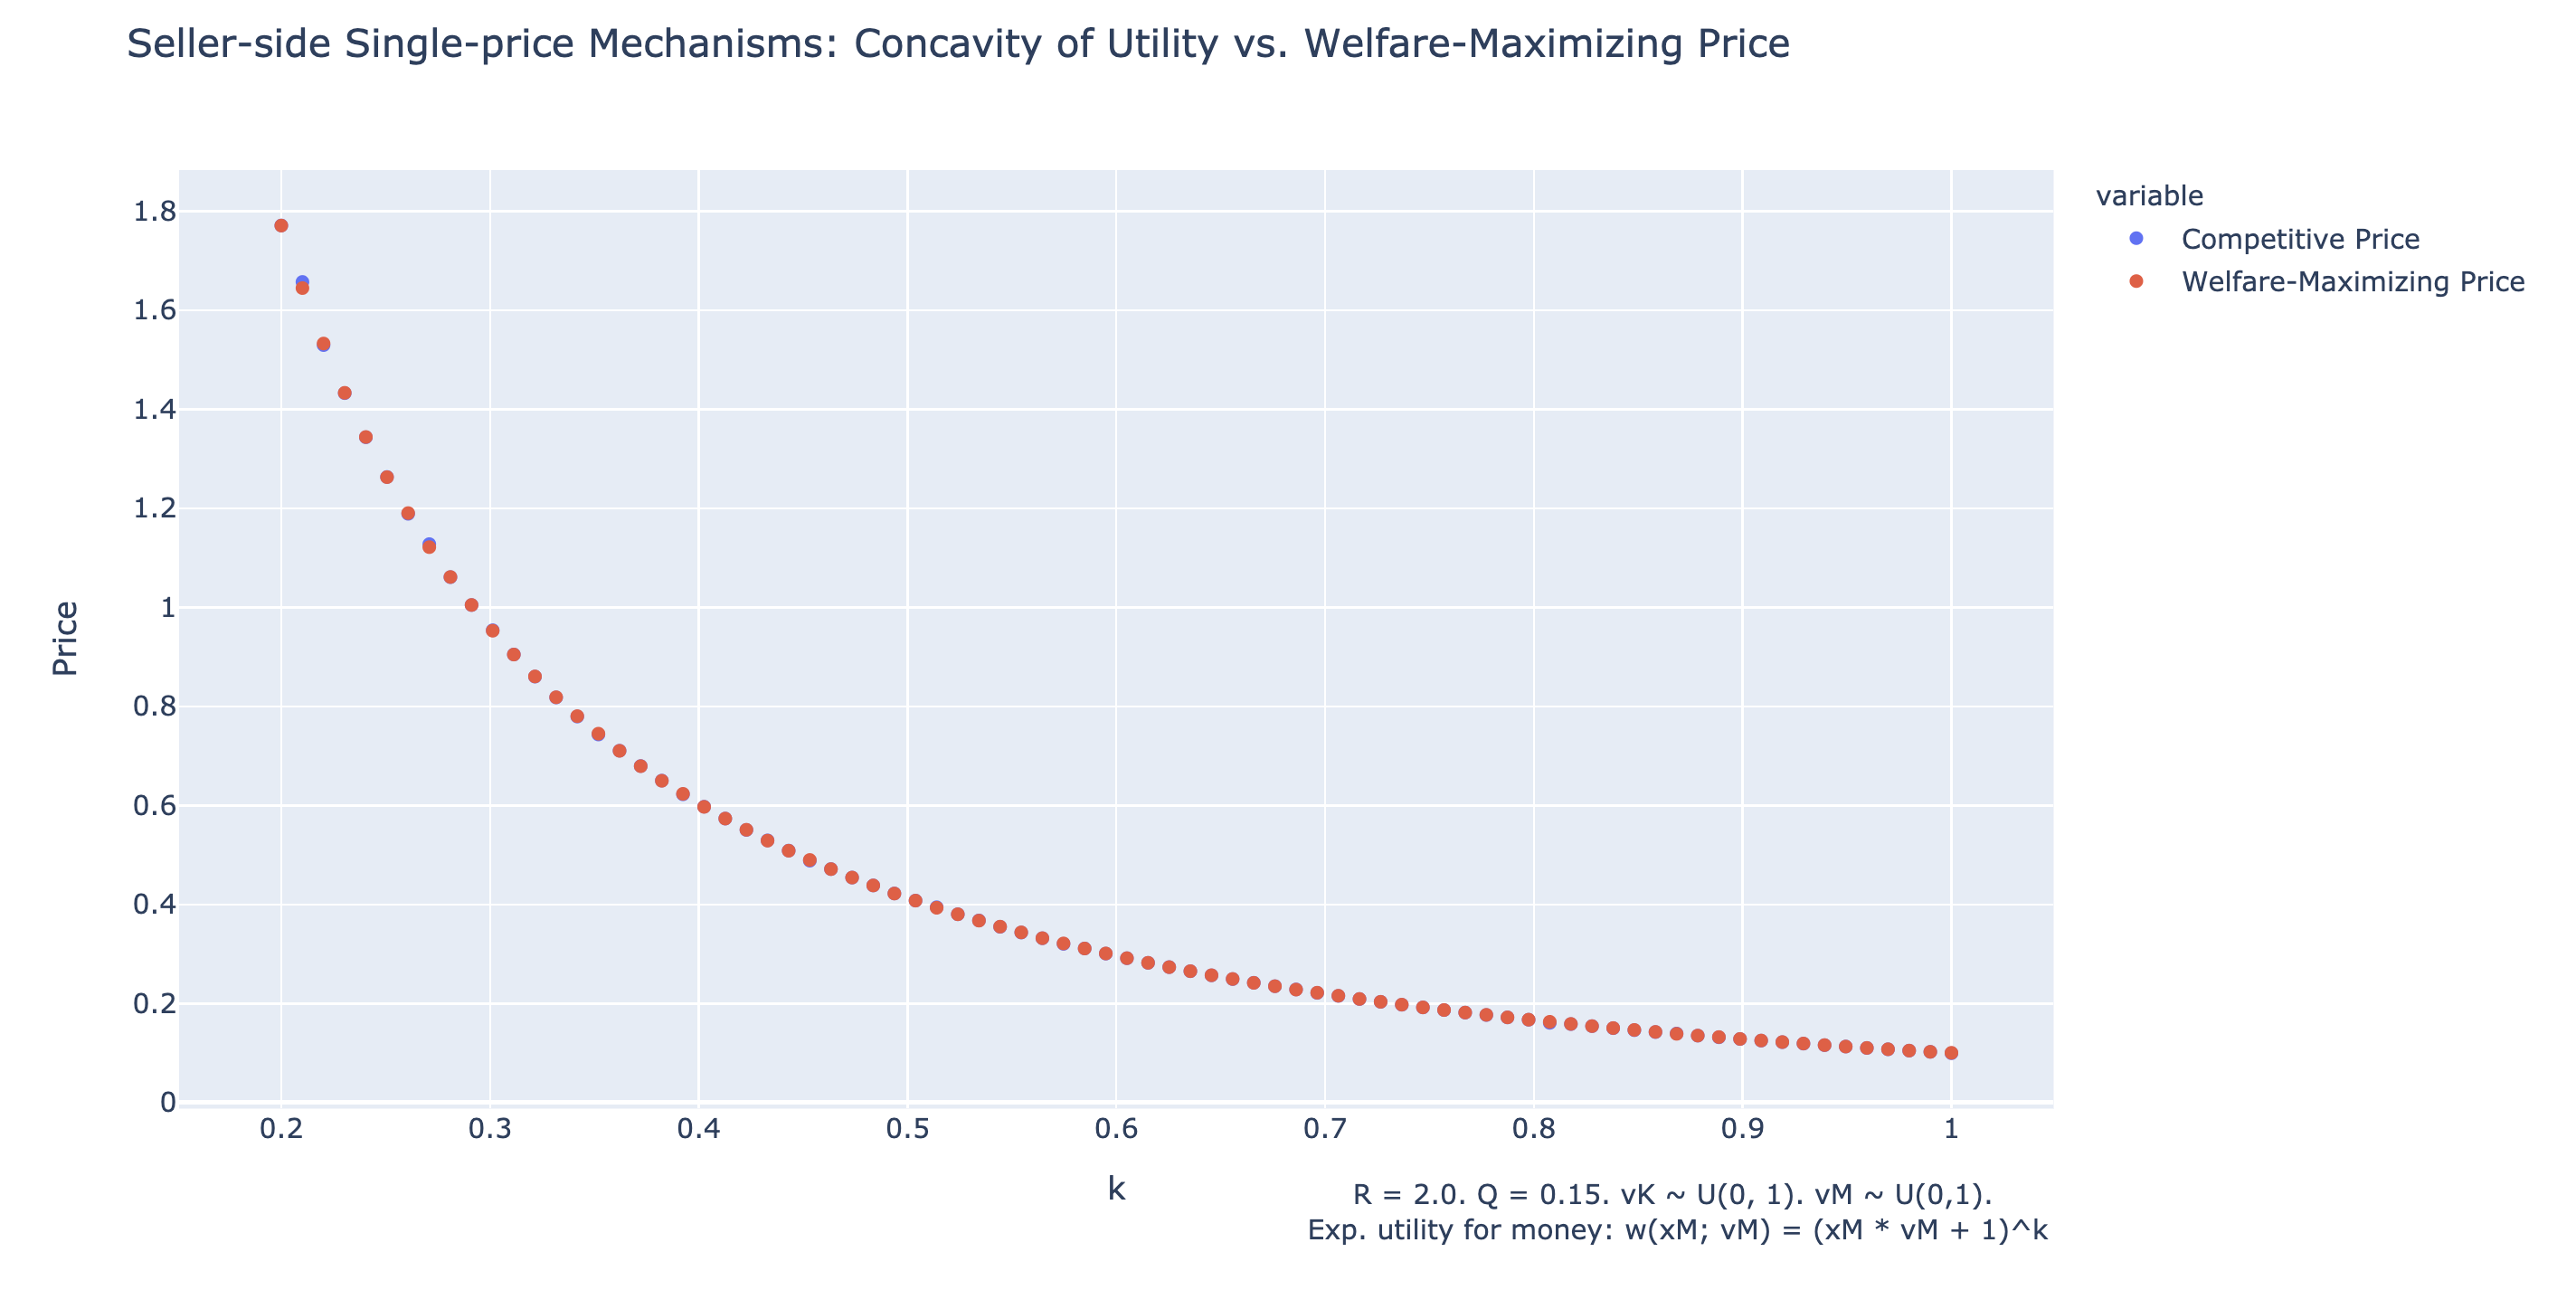
\includegraphics[width=\textwidth]{figures/k-vs-prices-inequality-low.png}
    \caption{Concavity of Utility (k) vs. Competitive Price and Welfare-Maximizing Price. Low-inequality setting.}
\end{figure}

Figure \ref{k-vs-prices-inequality-high} displays a setting in which inequality is high. In particular, we consider a setting where agents marginal utilities for the good are distributed as $v^K \sim U(0,1)$ and their marginal utilities for money are distributed as $v^M \sim \textrm{Pareto}(1/3)$. In this setting, when agents have linear utilities for money, the optimal mechanism is a single price above the competitive price, which results in rationing. In our numerical simulation, we find that when preferences are slightly concave, the optimal mechanism still utilizes rationing. When preferences are very concave, however, the optimal price coincides with the competitive price.

\begin{figure}
    \label{k-vs-prices-inequality-high}
    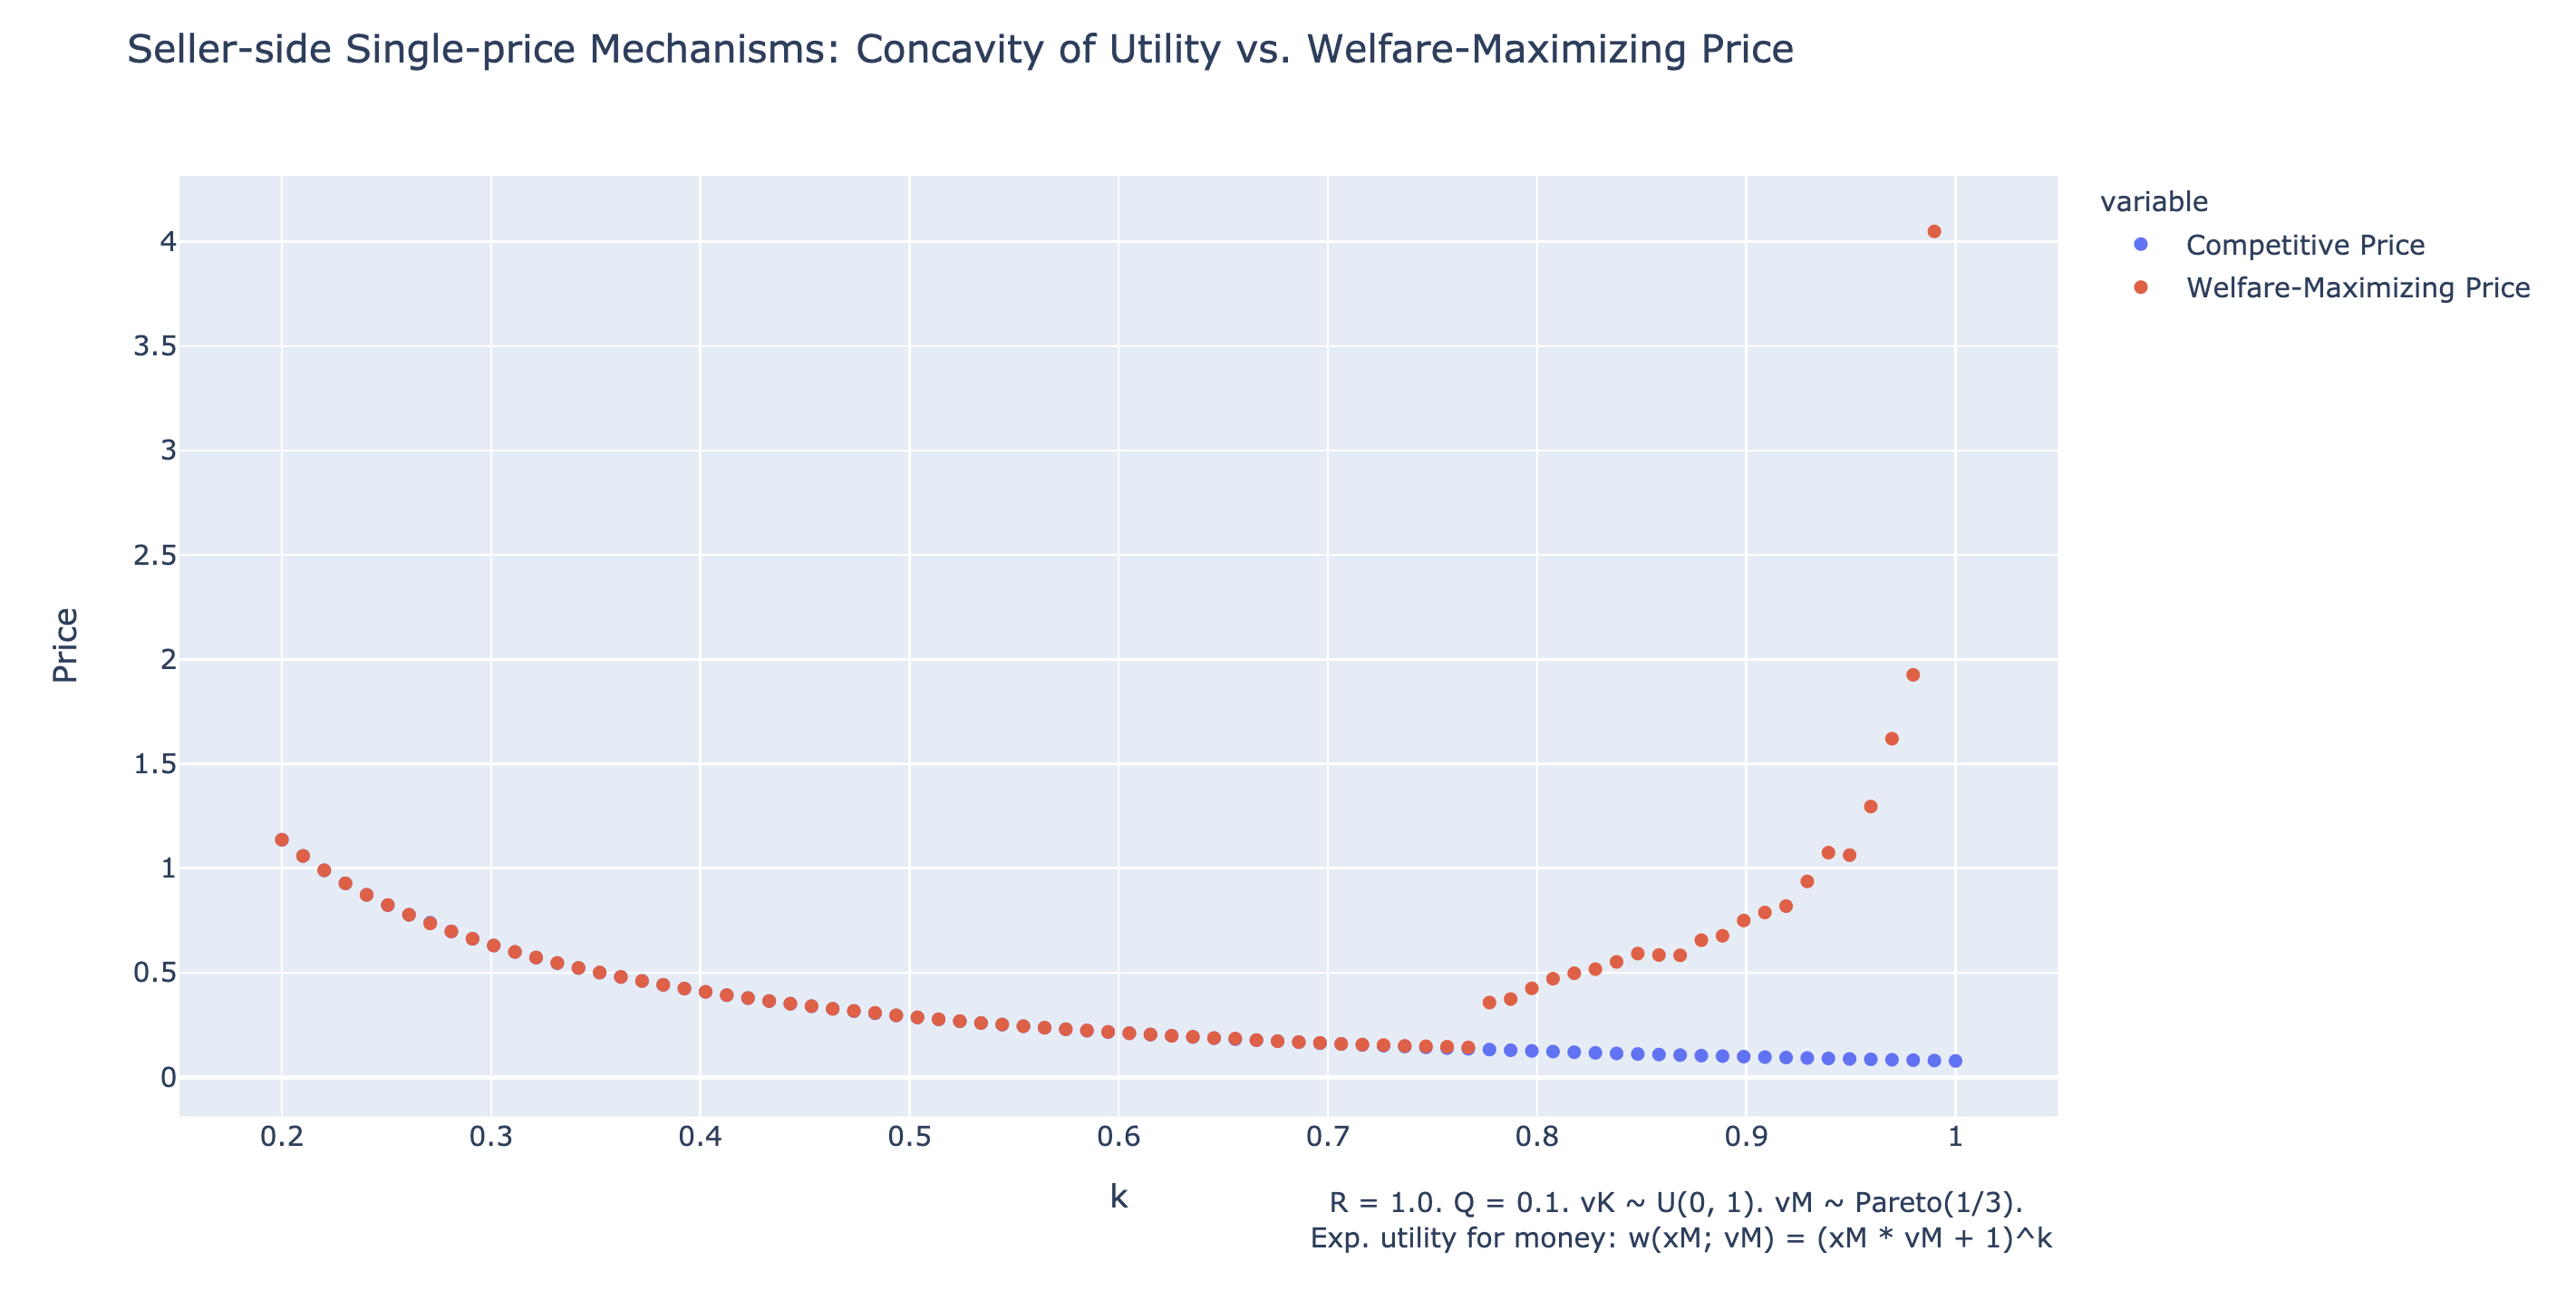
\includegraphics[width=\textwidth]{figures/k-vs-prices-inequality-high.png}
    \caption{Concavity of Utility (k) vs. Competitive Price and Welfare-Maximizing Price. High-inequality setting.}
\end{figure}

In both cases, we have only investigated two possible settings for the optimization problem, and we emphasize that it is an open question as to how much these results generalize to other settings.

\section{Conjectures}
\label{sec:conjectures}

Our work in the above sections suggest two corresponding analytic conjectures. First, our economic intuition in \ref{sec:economic-intuition} and our numerical simulations as in \ref{k-vs-prices-inequality-low} suggest that when the competitive price is optimal for the linear utility setting, it is also optimal in the concave-preference settings. Formally,\footnote{Note our slight abuse of notation in using $p_S^o(R, Q, F, w)$ to refer to the optimal price for utility function $w$ and using $p_S^o(R, Q, F, k)$ to refer to the optimal price when the utility function $w$ is parametrized by $k$.}

\begin{conj}
    \label{conj:competitive-price}
    Fix some revenue $R$, quantity $Q$, and valuation distribution $F$. Suppose that when agent preferences for money are given by $w(x^M; v^M) = x^M v^M$, we have $p_S^o(R, Q, F, w) = p_S^c(R, Q, F, w)$. Consider any agent preferences for money given by $\tilde{w}(x^M; v^M)$ with $\tilde{w}$ concave, increasing in $v^M$ and satisfying $\tilde{w}'(0) = v^M$. Then $p_S^o(R, Q, F, \tilde{w}) = p_S^c(R, Q, F, \tilde{w})$.
\end{conj}

Our second conjecture corresponds to the numerical simulation result in \ref{k-vs-prices-inequality-high}.

\begin{conj}
    \label{conj:rationing-robust}
    Fix some revenue $R$, quantity $Q$, and valuation distribution $F$. Consider the family of utility functions parametrized by $k$, with $w(x^M; v^M, k) = \frac{1}{k}(x^M v^M + 1)^k$. Suppose that $p_S^o(R, Q, F, 1) > p_S^c(R, Q, F, 1)$. Then there exists some $\varepsilon > 0$ such that $k \in (1-\varepsilon, 1]$ implies $p_S^o(R, Q, F, k) > p_S^c(R, Q, F, k)$. 
\end{conj}

If true, this conjecture would suggest that the use of rationing as found in \cite{dworczak-2020} is reasonably robust to the presence of risk-aversion among agents. When rationing is optimal for linear preferences, it is also optimal for slightly concave preferences.

\section{Future Work}
\label{sec:future-work}

More work is needed in three key directions: exactly characterizing the optimal mechanism for general concave preferences, characterizing optimality among all mechanisms, and extending this work to both sides of the market.

In the setting displayed in Figure \ref{k-vs-prices-inequality-high}, the welfare-maximizing price approaches the competitive price as preferences become more concave. However, more work is needed to verify exactly what the welfare-maximizing price is for various concave preferences. Alternatively, we could hope to find a threshold $k'$ for a given setting such that when preferences are sufficiently concave ($k < k'$), the competitive price must be optimal.

The second major area of extension is to generalize beyond single-price mechanisms to all possible mechanisms. We have covered only the first step in the analysis of \cite{dworczak-2020}, which considers single-price mechanisms as a preliminary case to general mechanisms. It is possible to imagine that concave preferences lead to more complex optimal mechanisms, even though \cite{dworczak-2020} find that optimal mechanisms generally take on a simple form. However, with general concave preferences, analytical approaches become particularly difficult. 

Finally, it remains to extend this work to a two-sided market, and solve for joint optimality in the market. We have analyzed only the seller-side of the market, in which poorer sellers are those more likely to want to sell. In the buyer side, willingness to buy identifies the opposite, identifying buyers with a higher value for money. This could lead to qualitatively different behavior.

There are also more open-ended extensions that would help determine acionable strategies in real world markets. Taking \cite{akbarpour-2020} as a departure point, one could incorporates externalities of the good's distribution into our optimization problem. Many public provisioning systems are also partially motivated by positive externalities, such as vaccine distribution, public housing, and public education, examples relevant to the work of \cite{kang-2020}.

% Perhaps: note that there are also other possible extensions, such as the use of a divisible good.

%  Other questions on the theme of ex-post fairness include the following (these are less concrete). Can we model the harm to poorer agents in this model that results from randomization? Can we develop a mechanism that ``trades off'' efficiency for less randomization? Could these answers change if the good is divisible? If this game is repeated, can we explicitly choose which agents are rationed to reduce ex-post unfairness? Are there established metrics of ex-post fairness which we can use to evaluate this metric?

% In a larger vein, it remains to model the markets of \cite{dworczak-2020} in conjunction with much of the literature on taxation and macroeconomic redistribution. What might happen if we have a government tax collector who can directly observe incomes, and another market designer (the subject of \cite{akbarpour-2020}) who cannot? How do their optimal mechanisms interact?

% Divisible good idea - Another approach is to change our model of the good. Can we improve on ex-post fairness when the good is divisible? In such a market, the designer would not be constrained solely to either giving each buyer a good or not giving them a good, but could distribute the good more evenly among these buyers. In such a market, instead of randomly choosing which of the rationed buyers are granted access to the market, the market designer might allocate smaller quantities of the good among those buyers, (hopefully) improving ex-post fairness. One might also hope to optimize such market designs based on measures of ex-post fairness, such as the minimal ex-post utility of all agents in the resulting market outcome. Examples of real-world market designs for divisible goods which are motivated by equity could include the provisioning of medical care, or rationing for limited supplies of food.

\section{Conclusion}
\label{sec:conclusion}

In this work, we analyzed the optimal single-price mechanism for maximizing total welfare in a setting where agents may have different marginal utilities for a good, and differing concave preferences for money. This setting is particularly relevant when designing price controls for labor markets. For example, when determining an appropriate minimum wage in a labor market, we should be concerned about wealth effects and agents' possible risk-aversion.

Our numerical simulation results validate this caution, while also showing that the use of rationing can be robust to slight concavity in agents' preferences. We generalize the method of \cite{dworczak-2020} to formulate a welfare-maximization problem for general agent preferences for money. We then numerically simulate how the competitive price and welfare-maximizing price change as preferences become more concave. We find that rationing may still be optimal when agents have slightly concave preferences for money. However, the welfare-maximizing price is closer to the competitive price than under linear preferences, and the two become equivalent when preferences are highly concave.

Further work is needed to analytically solve for the optimal price under general preferences, to generalize optimality to all mechanisms (not solely single-price mechanisms) and to extend our findings to a two-sided market. More broadly, the literature on redistribution through market design can benefit from a better understanding of how wealth effects shape optimal redistributive mechanisms. Precisely characterizing such mechanisms should yield designs that, when implemented, are more robust to preferences in the wild.

% Remove or comment out the next two lines if you are not using bibtex.
\bibliographystyle{aea}
\bibliography{inequality-design}

% The appendix command is issued once, prior to all appendices, if any.

\end{document}

